\section{What Physical Structure and Learned Features Recover}
\label{sec:evidence-bridge}

The continuous estimator builds on three distinct questions: what can be
reconstructed at unmeasured buses, what response distinguishes candidate
sources, and how evidence should be assigned when several explanations
fit. The following component experiments answer parts of these questions.
They use different cohorts and are not ablations of the final continuous
estimator. Figure~\ref{fig:evidence-bridge} places their measured effects
side by side without pooling their scores.

\begin{figure*}[t]\centering
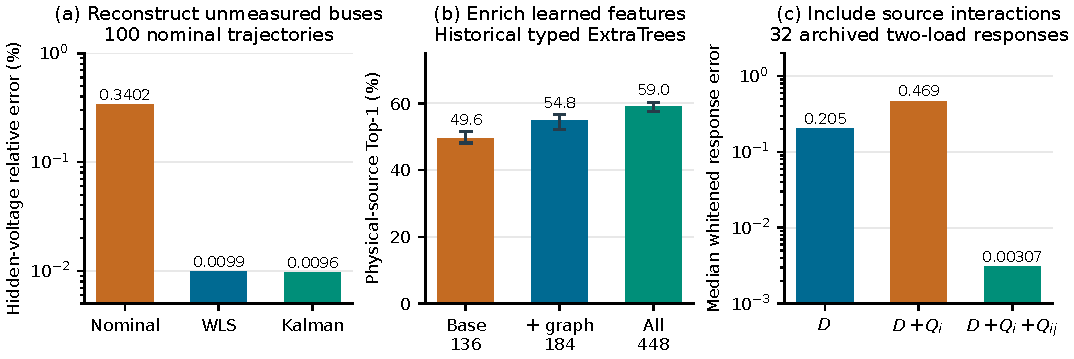
\includegraphics[width=.99\textwidth]{figures/generated/evidence_bridge.pdf}
\caption{Three separate component experiments. (a) Mean relative error of
the 31 unmeasured bus voltages under a matched nominal model; this is not a
PMU compliance TVE test. (b) Mean physical-source Top-1 over three model
seeds, each scored on 7,915 labeled physical samples, in the historical
typed-ExtraTrees feature study; whiskers show the
seed range, not a confidence interval. These 136--448-feature models are
neither the final hackathon submission nor the causal comparators.
(c) Median whitened prediction error at the archived 120-report horizon
for two-load responses: mixed-source terms matter, while adding only
self-curvature worsens this metric. Each panel has its own units and cohort.}
\label{fig:evidence-bridge}\end{figure*}

\subsection{Recovering Unmeasured Voltages Is Not Yet Event Attribution}
In 100 nominal test trajectories, the mean hidden-voltage relative error
falls from \BridgeNominalError\% for the equilibrium reference to
\BridgeWLSError\% for snapshot weighted least squares and
\BridgeKalmanError\% for a causal Kalman reconstructor. Most of this
improvement comes from conditioning the physical network on the measured
phasors; temporal filtering adds a smaller improvement. This supports
reconstruction under that model and sensor placement, not unique recovery
of every source. The independently evaluated Kalman reconstructor is not
silently substituted for the conditional observer in the main article.

\subsection{Physical Features Remain a Useful Learned Route}
The historical feature study raises physical-source Top-1 from
\BridgeBaseTop\% with 136 features to \BridgeGraphTop\% with graph-temporal
features added, and \BridgeFullTop\% with the full 448-feature set.
Voltage level, relative angle, frequency, time scale and spatial coherence
carry complementary information; Fig.~\ref{fig:evidence-bridge}(b) reports
an executed feature comparison rather than an inferred explanation of
tree importance. Electrical features make a classifier physics-informed
in its representation. They do not enforce Kirchhoff balance on its
predicted label or compute the PMU response of a candidate intervention.

For phase-to-neutral RMS phasors and a declared current orientation,
\begin{equation}
 S_{ij}=P_{ij}+\mathrm jQ_{ij}
       =\sum_{\phi\in\{a,b,c\}}V_{i\phi}I_{ij,\phi}^{*}.
 \label{eq:bridge-terminal-power}
\end{equation}
This expression requires voltage and current at the same terminal.
In the frozen map, the bus-2 voltage is paired with a current measured at
bus 3, and the bus-10 voltage with a current at bus 11. Their raw channel
products are therefore power proxies, not exact terminal powers. Even a
co-located terminal power is not the bus's net injection unless all
relevant terminals are accounted for. Frequency and ROCOF complement the phasors
but share the instrument's angle processing; the likelihood must account
for that dependence. Fundamental-frequency phasors also do not determine
harmonic distortion. Thus adding nominally physical features does not
by itself supply missing harmonic or nodal-injection measurements.

\subsection{Mixed-Source Response Coefficients}
For simultaneous load changes, a second-order response approximation
includes products of the input amplitudes. In the archived two-load
experiment,
\begin{equation}
 s_{q,n}(a)=\sum_i D_{qni}a_i+\sum_i Q_{qni}a_i^2
               +\sum_{i<j}Q_{qnij}a_ia_j,
 \label{eq:bridge-response-tensor}
\end{equation}
where $q$ indexes PMU coordinates, $n$ elapsed reports and $i,j$ load
sources. Centered nonlinear simulations estimate the coefficients; the
$Q$ terms include their Taylor scaling. The mixed term represents the
interaction of two simultaneous load changes. Across 32 archived
two-source responses, median whitened error is \BridgeDError{} for $D$,
\BridgeQError{} after self-curvature, and \BridgeMixedError{} after mixed
terms. This is evidence for response fidelity in that local experiment.
It is not a measured classification gain from inserting this second-order
tensor into the continuous load/line bank, which uses switched local
predictors instead.

The coefficients in \eqref{eq:bridge-response-tensor} form a tensor over
measured coordinate, elapsed time and source indices. The useful term is
the physical cross-source interaction $Q_{qnij}$; the array's shape alone
does not provide an accuracy or computational advantage.
In the continuous estimator, $M$ is instead a vector of aggregated
source/family weights at each report, and $\Delta M$ is its temporal
difference, as defined in the main article.
That implementation does not require a tensor decomposition or a
tensor-learning library.

\subsection{Why Integrate Severity Rather Than Select the Best Fit?}
An extra source with zero amplitude can reproduce a smaller source set.
Best-fit residual alone therefore cannot decide cardinality. In the
archived load-support estimator, the model-selection quantity is
\begin{equation}
 Z_S=\int p(r\mid s_S(a),\Sigma)p(a\mid S)\,da,
 \qquad p(S\mid r)\propto Z_Sp(S).
 \label{eq:bridge-batch-evidence}
\end{equation}
Integration accounts for the prior volume of amplitudes consistent with
the data, rather than rewarding only the best-fitting amplitude. This is
standard Bayesian model comparison applied to an electrical response
model, not a new Bayes rule. The archived implementation evaluates the
null, 16 single-source and 120 pair supports with 31-point Gauss--Hermite
quadrature per amplitude. Table~\ref{tab:archived-support-bridge} shows
both its successes and its loss of resolution for weak sources.

\begin{table}[t]\centering\small
\caption{Archived joint cardinality-and-support decisions. Onset, load
family and operating context are supplied. These are noise replays of
shared physical trajectories, not independent continuous detections.}
\label{tab:archived-support-bridge}
\begin{tabular}{@{}lrr@{}}\toprule
Amplitude regime & Replays & Joint support Top-1 \\\midrule
Finite / finite & 1,440 & 100.00\% \\
Moderate / moderate & 1,440 & 98.82\% \\
Weak / strong & 1,440 & 66.25\% \\
Weak / weak & 5,760 & 24.38\% \\
\bottomrule\end{tabular}

\end{table}

An audit found a one-source evidence normalization offset in this
archive: the implemented cardinality prior is proportional to
$(0.20,0.50/(2\pi),0.30)$ rather than the declared $(0.20,0.50,0.30)$.
The table preserves the executed results under that effective prior;
it does not validate calibrated posterior probabilities or a corrected
replay. The continuous estimator uses separate, independently checked
local evidence code. Consequently these component results motivate the
physical/Bayesian construction, but do not establish that adding Bayes
or tensor storage alone causes its final accuracy advantage.
